\section{Internet - practical aspects}

While the important theoretical aspects of the internet have been discussed in the section \emph{networking}, there are so many important details that we devote another section purely to those. 

\subsection{Nomenclature}

\begin{itemize}
	\item url
	\item uri
	\item domain
	\item 
\end{itemize}




\subsection{Session basics}

software:
     node: client-sessions (good crypto)
     bcryptjs for hashing
     csurf for CSRF


http session
    http: Since http is a stateless protocol, we need some helper to store state over several page-visists
    session: webserver tells browser to remember the user
           http-response-header: "Set-Cookie": "session=12345"
           cookies:  server stores information here
                          that info is sent with every http-request's header
                          "Cookie": "session=12345"
                         Cookies are stored in the browser in a secret spot (not the usual browser-cache or db). They are only sent to a site if the sites url matches the cookie-domain. This means that sites cannot see cookies from other sites.
                   client-sessions has some very recomended headers for cookies:
                        httpOnly: true // dont let js access cookies
                        secure: true // only set cookies over https
                        ephemeral: true // destroy cookies when browser closes

storing passwords:
    passwords must be hashed.


SSL/TLS
     Those cookies are just strings in the HTTP-header! They can be stolen! So they need to be encrypted.
     What is not encrypted by ssl?
           SSL does encrypt everything, except ...
                       the initial handshake target (ie your banks url)
                       every requests url 
             but it *does* encrypt all headers (hence cookies), and post- *and* get parameters.
      



Tokens:(more specifically, JWT, OR, a bit more extensive, OAuth2. Not to be confused with USB-stick tokens)
     Originally, tokens were designed as an alternative to cookies that would also work in apps.
     Based on this, however, two protocols (JWT and OAuth) grew, that go beyond what you could do with cookies. 
    Here's what you cannot do with cookies. They are a two-party thing. 
       - they are bound to a single domain. but your app might have multiple backend-services.
     OAuth/JWT is for multi-party things.
     JWTs are like a Vollmacht: 
        -  your app (tinder) wants to access your facebook photos
        - you login at facebook to tell it that tinder may use those photos
        - facebook gives you a token that reads: {"photoPermission": "1234!"§$"}
        - you pass that token to tinder
        - tinder sends the token to facebook
        - facebook verifies that you have indeed given that permission
        - facebook gives tinder the photos
     Technically, they are commonly implemented as a special type of cookie.
            But they could be implemented as Post-Header + localStorage, too. 
            (more-often so, actually, because contrary to browsers, mobile-apps don't know about cookies)
     Some more stuff:
           cookies usually contain any information that some programmer deemed necessary.
           tokens follow strict standards (JWT or OAuth)
           Tokens usually don't require tinder to maintain a session in its database (though they might)
                But does facebook still need to maintain a session?
           Tokens don't require a remote-session because the token contains user-data. 


\subsection{Authentication, SSO, and authorization}
Information from \href{https://www.varonis.com/blog/what-is-oauth/}{here}.
Assume that you want to check the identity of a user. That user is already member of some authentication-service like facebook. You could ask the user for his facebook-password. But authenticating at some place with your password is insecure, because your password needs to make it over the network. Instead, the user can ask facebook for a token, pass it to your site and you then check with facebook if this token is cool. 
Strictly speaking, OAuth is about authorisation (is the user allowed to use my service?), not about authentication (is the user really Michael?). The common analogy I’ve seen used while researching OAuth is the valet key to your car. The valet key allows the valet to start and move the car but doesn’t give them access to the trunk or the glove box. An OAuth token is like that valet key. As a user, you get to tell the consumers what they can use and what they can’t use from each service provider. You can give each consumer a different valet key. They never have the full key or any of the private data that gives them access to the full key.
           
           

\begin{table}[]
     \begin{tabular}{@{}lll@{}}
     \toprule
                                             & Centralized                                                                                                                                                                          & Decentralized                                                                                                                                                                                                                                 \\ \midrule
     \multicolumn{1}{|l|}{Authorization}  & \multicolumn{1}{l|}{CAS has an extension for authorization.}                                                                                                                            & \multicolumn{1}{l|}{\begin{tabular}[c]{@{}l@{}}OAuth2:\\ The user tells your app and a second app\\ what your app may do on second app on his behalf\end{tabular}}                                                                            \\ \midrule
     \multicolumn{1}{|l|}{Authentication} & \multicolumn{1}{l|}{\begin{tabular}[c]{@{}l@{}}CAS:\\ your backend verifies that the user is really him\\ \\ (backend may be one of Kerberos, LDAP or ActiveDirectory)\end{tabular}}    & \multicolumn{1}{l|}{\begin{tabular}[c]{@{}l@{}}OpenId:\\ A usage of OAuth2 for authentication.\\ The user tells your app on which second app you can get proof \\ that the user is really him\\ \\ Example: Sign-in-with-github\end{tabular}} \\ \bottomrule
     \end{tabular}
\end{table}
To confuse things a little, some CAS Implementations also support OAuth.


\subsection{Security threats}


CSRF
    someone makes you click a link that is actually a form-post.
    Counter meassures:
       additionally to the session-cookie, we create a token for every page-load.
       token provided by server
       token added to form (as hidden field)
       token sent back with form when user hits submit
       server compares form-token with given token
        if not identical, then 
            some bad guy sent us a link that we didn't


XSS


% Please add the following required packages to your document preamble:
% \usepackage{booktabs}
\begin{table}[]
     \begin{tabular}{@{}lll@{}}
     \toprule
               & XSS: evil code being sneaked into frontend                                                              & XSRF: evil request being sneaked into backend                                                                                                                                                                     \\ \midrule
     Roles     & User trusts compromised site                                                                            & Site trusts mislead user                                                                                                                                                                                          \\
     Mechanism & Attacker injects script into site                                                                       & Attacker tricks user into issuing request                                                                                                                                                                         \\
     Method    & Attacker posted a comment that was not properly validated and now displays evil scripts to another user & Attacker made user click on something that causes a request to the backend                                                                                                                                        \\
     Counters  & Form validation: don't allow script tags and similar in posts.                                          & \begin{tabular}[c]{@{}l@{}}Form-tokens: a form-post must have been expected by backend (prevents evil email-links)\\ Cors: a form-post can only come from backend's own domain (prevents evil twins)\end{tabular} \\ \bottomrule
     \end{tabular}
\end{table}


\paragraph{CORS} (cross origin resource sharing) is the act of one site (www.mysite.com) requesting data from another, third-party site (www.puppyimagehost.org?img=3241). Doing so is forbidden by default, and browsers will block such requests. The reason is that a hacker could use his browser to do something malicious. This here is a perfectly fine request: 
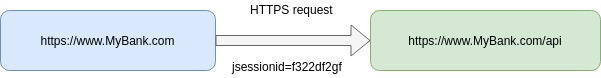
\includegraphics[width=0.7\textwidth]{images/cookie_3.jpg}
After that request, the \inlinecode{jsessionid} cookie will be stored on the browser. A hacker could now steal that cookie and do this: 
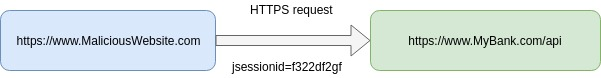
\includegraphics[width=0.7\textwidth]{images/cookie_4.jpg}
This is called Cross-site-request-forgery. Honestly, it seems that this is something that should be fought on the \emph{sever}side, not from the client.


However, some sites depend on CORS.
\begin{itemize}
	\item For one, images and scripts can be loaded from third-party sites (using the \inlinecode{src} attribute). As such, for historical reasons, images are exempt from CORS-blocking
	\item Maybe www.puppyimagehost.org \emph{wants} to expose an API for other sites to call. In this case, www.puppyimagehost.org can set an additional header on its response: \inlinecode{Access-Control-Allow-Origin: www.mysite.com} or \inlinecode{Access-Control-Allow-Origin: *}
\end{itemize}
Note that there is no way that www.mysite.com can deactivate CORS-blocking; it \emph{must} be allowed by www.puppyimagehost.org. An individual person might deactivate the browsers CORS-settings (if the browser allows you to do that), but the common user will never do that. 

\paragraph{CORS when applied to an OL-canvas} Really, using 3rd party data is a bit like a one-night-stand: you need consent from both sides. The server gives consent to the usage of its images by setting \inlinecode{Access-Control-Allow-Origin}, the client does so by setting \inlinecode{crossorigin="Anonymous"} (or \inlinecode{crossorigin="use-credentials"}). 
Now a canvas is a special case. For one, often we load images from more than one external source, so we need to get two-way-consent with a whole series of services. On the other hand: even if we don't actively set \inlinecode{crossorigin}, data is displayed - errors only start to occur once we want to call \inlinecode{canvas.toDataUrl(...)}. Why is that? Well, canvases load \inlinecode{img}'s, and those are, as mentioned above, exempt from CORS-restrictions by default. However once we want to do any manipulations on that data, CORS kicks in again.
That is why you can show any layer on a canvas, but cannot export it to pdf as long as it displays any layer that does not have two-way-consent.

\paragraph{CORB} (cross origin read blocking) is when your browser deletes a request's response body before it can be red by your site. This is to prevent www.puppyimagehost.org from accidentially leaking sensitive information.
Even with CORS, an attacker might use html tags like \inlinecode{img} to circumvent CORS-blocking. This is not a case of cross-site scripting, but rather of building a malicious website from scratch just to sneakily access data.
\begin{itemize}
	\item First, load remote data to its site using \inlinecode{<img src="https://your-bank.example/balance.json">} or \inlinecode{<script src="https://your-bank.example/balance.json"></script>}
	\item The browser would notice that the data in \inlinecode{src} is not an image (or javascript) and consequently would not display the data as image. 
	\item But the browser \emph{would} still have the data in it's memory. The attacker can then use a browser-memory vulnerability like spectre to access this data. 
\end{itemize}

Let’s break down how CORB works. A website can request two types of resources from a server:
\begin{itemize}
	\item data resources such as HTML, XML, or JSON documents
	\item media resources such as images, JavaScript, CSS, or fonts
\end{itemize}
A website is able to receive data resources from its own origin or from other origins with permissive CORS headers such as \inlinecode{Access-Control-Allow-Origin: *}. On the other hand, media resources can be included from any origin, even without permissive CORS headers.

CORB will block the response of a request if all of the following are true:
\begin{itemize}
	\item The resource is a "data resource". Specifically, the content type is HTML, XML, JSON
	\item The server responds with an X-Content-Type-Options: nosniff header, or if this header is omitted, Chrome detects the content type is one of HTML, XML, or JSON from inspecting the file
	\item CORS does not explicitly allow access to the resource
\end{itemize}

CORB protects neither against XSS nor XSRF. Instead, it prevents one mechanism of side-channel-attacks.

